\documentclass[a4paper,12pt]{article}
\usepackage{cmap}
\usepackage[cp1251]{inputenc}
\usepackage[english, ukrainian, russian]{babel}
\usepackage[left=2cm,right=1.5cm,top=1cm,bottom=1cm]{geometry}
\usepackage{amssymb}
\usepackage{graphicx}
\usepackage{listings}

\begin{document}

\pagenumbering{gobble}


\begin{large}

\begin{center}
\section*{GraphQL.}
\end{center}

\medskip

\section{Welcome to GraphQL}

GraphQL, often dubbed as a query language for APIs, allows clients to request exactly the data they need, no more and no less. Unlike REST APIs, where endpoints dictate the structure of the response, GraphQL empowers clients to define their data requirements through queries. This level of control eliminates over-fetching and under-fetching of data, streamlining network requests and enhancing application performance.

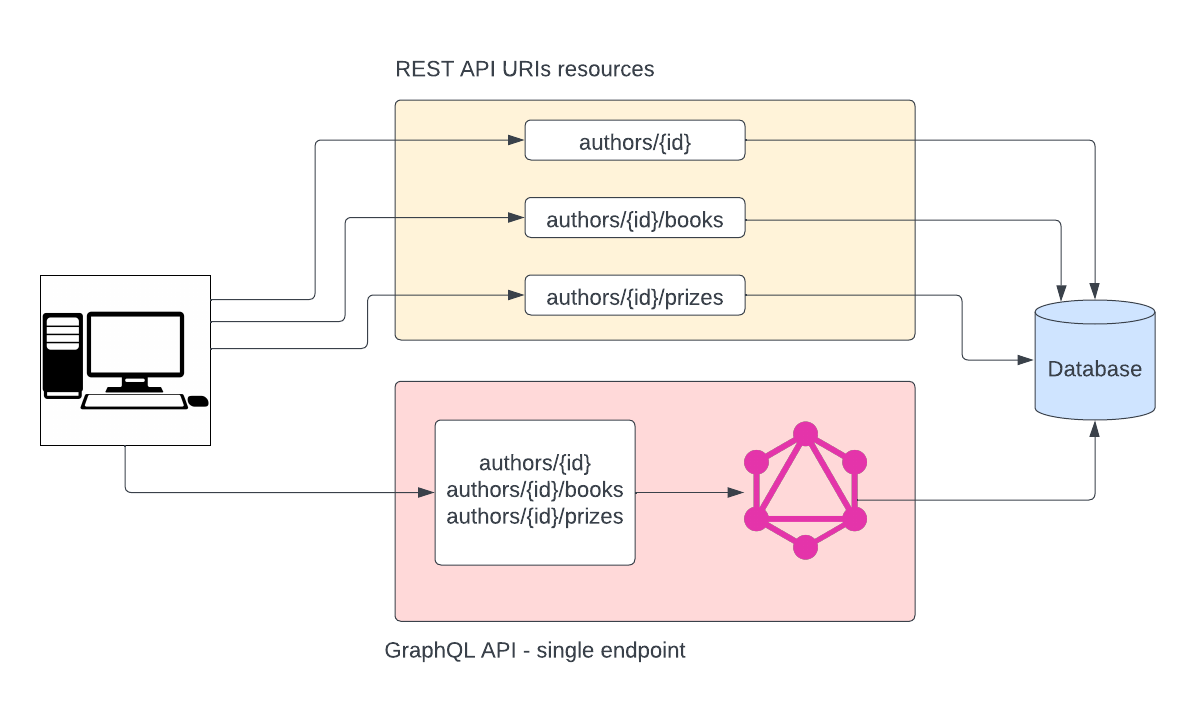
\includegraphics[scale=0.8]{gq1}

\section{GraphQL vs REST}

Advantages of GraphQL

\begin{itemize}
\item Efficiency in Data Retrieval: GraphQL enables clients to request precisely the data they need, minimizing over-fetching or under-fetching of information. This tailored approach enhances performance and reduces unnecessary network traffic, ultimately resulting in faster response times.

\item Single Request, Multiple Resources: Unlike REST, which often necessitates multiple endpoints for different resources, GraphQL allows clients to retrieve related data in a single request. This reduces the infamous "N+1 query" problem and simplifies data aggregation.

\item Flexible Schema Evolution: GraphQL's schema-first design empowers developers to evolve APIs without breaking changes. New fields and types can be added without impacting existing clients, fostering agility and accommodating changing business requirements.

\item Strongly Typed: GraphQL enforces a strongly typed schema, providing clear definitions of available data and operations. This eliminates ambiguity and reduces runtime errors, leading to more robust and maintainable codebases.
\end{itemize}

Disadvantages


\begin{itemize}
\item Complexity in Caching: Caching in GraphQL can be more challenging due to the dynamic nature of queries. Implementing efficient caching strategies requires careful consideration and additional effort.

\item Potential for Over-Fetching: While GraphQL's flexibility is an advantage, inexperienced or poorly optimized queries might still lead to over-fetching of data, impacting performance.
\end{itemize}


\section{Queries and Mutations}
 
In GraphQL, queries and mutations are two fundamental operations that clients can use to interact with the server and retrieve or manipulate data. They serve distinct purposes and are designed to facilitate efficient and flexible communication between clients and the GraphQL server.

\textbf{Queries}: Queries in GraphQL are used to request data from the server. They resemble a data structure that defines the shape and structure of the data the client is interested in fetching. With queries, clients can specify exactly what fields they need, allowing them to retrieve only the necessary data and avoid over-fetching.

\textbf{Mutations}: Mutations in GraphQL are used to modify data on the server. They provide a way for clients to create, update, or delete data. Mutations are similar in structure to queries but are executed with the intent of making changes to the data on the server.

The query type in GraphQL represents a read-only view of all of our entities and ways to retrieve them. A query type is required for every GraphQL server.




\end{large}
\end{document}

